\documentclass{report}
%\usepackage{includegraphicx}
\usepackage{sydewkrpt}
\usepackage{longtable}
\usepackage{array}
\usepackage{ragged2e}
\usepackage{amsmath}
\usepackage{amssymb}
\setcounter{secnumdepth}{5}
\setcounter{tocdepth}{5}
\DeclareMathOperator*{\argmin}{\arg\!\min}
\DeclareMathOperator*{\argmax}{\arg\!\max}
\newcolumntype{P}[1]{>{\RaggedRight\hspace{0pt}}p{#1}}

%%%%%%%%%%%%%%%%%%%%%%%%%%%%
%%%    Begin Document    %%%
%%%%%%%%%%%%%%%%%%%%%%%%%%%%
\begin{document}
\pagenumbering{roman}

\waterlootitle{SYDE 462: Spring Term Final Report}{
  Group 2: Relay \\
  Adaptive Traffic Control Framework
}{
  Alex Huras -- 20344660\\
  D. Scott Neil -- 20349210\\
  Myles Tan -- 20349217\\
  Riley Donelson -- 20342815\\
  }

\dotableofcontents

\newpage
\doublespacing
\pagenumbering{arabic}

\chapter{Background Information}
\setlength{\parindent}{1cm}

\newpage

\subsection{Front End}
\chapter{Engineering Design}

\section{Design Process}
With sufficient Design Research conducted, and functional requirements compiled, the front-end application design moved into an iterative process of defining the user interface (UI), interactions, and visual design of the app through various levels of fidelity.
The use of many design tools was employed, as best suited for each given stage of the design process. 
These tools include Adobe Photoshop and Illustrator, HTML/CSS/JavaScript, and sketching using pencil and paper to quickly illustrate low-fidelity ideas.

\subsection{Wireframing}
The process began with a wireframing stage, involving the quick iteration of information architecture and UI techniques, to discover optimal implementations for each of the functional requirements.
Global app navigation, page layout, modularity, and fundamental UI elements were initiated at this stage, to begin to define the design language used in the application.
This was accomplished mainly through static paper-based sketches of various screens.
This allowed for rapid generation of concepts, and movement between and through ideas. 

\begin{figure}[htbp!]
  \begin{centering}
    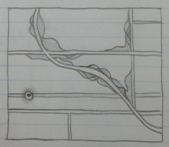
\includegraphics[scale=1]{figures/wire-1.png}
    \caption{Initial wireframe for histogram approach.}
    \label{fig:wire-1}
  \end{centering}
\end{figure}

\begin{figure}[htbp!]
  \begin{centering}
    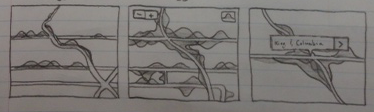
\includegraphics[scale=1]{figures/wire-2.png}
    \caption{Application wireframes showing interaction controls and pop-up menu.}
    \label{fig:wire-2}
  \end{centering}
\end{figure}

As can be seen in Figures \ref{fig:wire-1} - \ref{fig:wire-4}, various overlay techniques using both histograms and circular polygons on a map of a city were explored here in this early stage.
The histogram approach sought to model each vehicle (or small group of vehicles) on the road as a probability density function that could be moved along a road based on knowledge of traffic presence at each intersection, and speed limit data on each road.
More vehicles means more histograms, shown as translucent graphs which when overlaid, become more and more opaque, thus indicating a higher traffic density in that area.

\begin{figure}[htbp!]
  \begin{centering}
    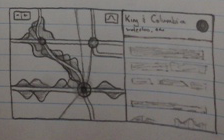
\includegraphics[scale=1]{figures/wire-4.png}
    \caption{Sketch of potential side menu for the Relay Interface application.}
    \label{fig:wire-3}
  \end{centering}
\end{figure}

Response for this concept was generally critical, as probability functions overlaid on a map were found to not be particularly easy to understand, at least not immediately at a glance.
It was evident at this stage that a simpler - more intuitive - visualization was needed for this application to be useful for both consumers and traffic engineers.\\

\begin{figure}[htbp!]
  \begin{centering}
    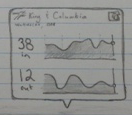
\includegraphics[scale=1]{figures/wire-5.png}
    \caption{Sketch of a detailed pop-up menu showing intersection data.}
    \label{fig:wire-4}
  \end{centering}
\end{figure}

Through exploration of the circular polygon heat-map concept, a more agreeable solution was found.
This concept modelled traffic data on a per intersection basis.
In other words, when an intersection is experiencing a high volume of traffic, a translucent circular polygon is triggered and overlaid onto a map of the city at the longitude and latitude of the intersection.
The size of the circle is positively correlated to the volume of traffic at the intersection.
A second degree of data is then shown through use of colour, to illustrate the performance of the intersection itself.
This gives insight into how well the intersection is moving traffic given it's high-volume state.
It was agreed upon that a well-performing high-volume intersection should receive a colour that is neutral, while a high-volume intersection with poor performance should emit a colour that indicates that something is wrong, such as orange or red.

It can also be seen in the figures that other components of the prototype application were accounted for in the wireframes.
These include interactions such as pop-up dialogues, highlighting routes and communicating intersections, as well as a side-panel for showing detailed metrics on intersection and overall city-wide traffic performance.
From this stage, the prototype moved to a mid-fidelity phase to further build out the concepts and refine the aesthetic of the application.

While not all of these early-stage concepts were used in the final product, the process of generating, critiquing, and refining multiple ideas proved valuable throughout the year.
These initial visualization concepts helped to spawn and guide future implementations, and helped attain a clear understanding of the data being presented.
The next step in the design process moved into a medium-fidelity stage, such that navigation and interaction could be explored at a deeper level.

\subsection{Medium-Fidelity Prototyping}
Through the use of prototyping software Balsamiq, a set of interactive mockups were created to both reflect the requirements of the application, as well as ideas and lessons learned from the previous wireframing stage.
In this prototype, the main tenets for the final version of the application were created in an illustrative form, to identify key architectural components and the user's interaction within.
By doing this in a medium that does not put too much focus on the specifics of visual design, it was easier to concentrate on the core features of the application, and how they satisfy (or dissatisfy) the original requirements. 

At this stage, the concept of data layers was explored.
Given that there are many varying metrics identified as important to target users (Traffic Engineers), and that these metrics all have a spatial or location-based relevance, the idea of turning on and off layers of data visualization overlaid on a map was critical in effectively demonstrating traffic data.
Metrics such as intersection Status, and Flow through an intersection were conceptualized at this stage, with some preliminary UI put together for interacting with these layers.
A screenshot of the mockup showing a Status visualization in the Relay app is presented in Figure \ref{fig:bals-1}. \\

\begin{figure}[htbp!]
  \begin{centering}
    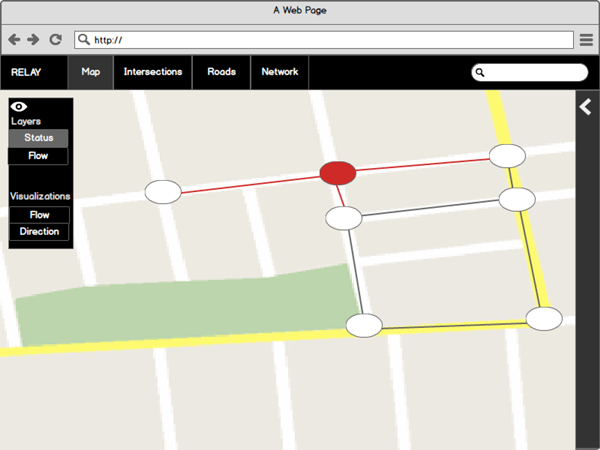
\includegraphics[scale=0.6]{figures/bals-1.png}
    \caption{Balsamiq mockup of a data layer in the Relay app.}
    \label{fig:bals-1}
  \end{centering}
\end{figure}

Additionally, as can be seen at the top of Figure \ref{fig:bals-1} the foundations for global app navigation were built out, in the form of a fixed header bar at the top of the screen.
This header serves many purposes, including branding for the app, search functionality, as well as tabbed buttons to move between contextually grouped pages.
Figure \ref{fig:bals-1} shows the active state of the Map button, while the main area of the screen contains a map with relevant data.

Further interaction design was carried out at this stage, in the form of a modular popup window, referred to as the Relay info box.
This info box was designed to present deeper metrics for an intersection, and appears when an intersection on the map is clicked.
This allows users to quickly inspect any intersection of interest and monitor time-series data in the context of a specific location.
Data provided at this stage includes a graph of the flow of traffic through the intersection in each of the cardinal directions, as well as a matching chart that provides predictive data into the near future, based on stochastic methods from the controller.
The status of the lights is shown, in addition to numerical car counts and the name of the intersection that has been clicked.
A Balsamiq mockup of the info box is presented in Figure \ref{fig:bals-2}. \\

\begin{figure}[htbp!]
  \begin{centering}
    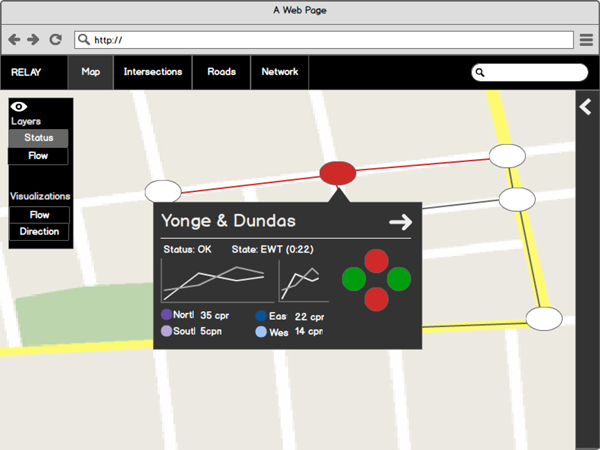
\includegraphics[scale=0.6]{figures/bals-2.png}
    \caption{Balsamiq mockup of the Relay info box.}
    \label{fig:bals-2}
  \end{centering}
\end{figure}

\begin{figure}[htbp!]
  \begin{centering}
    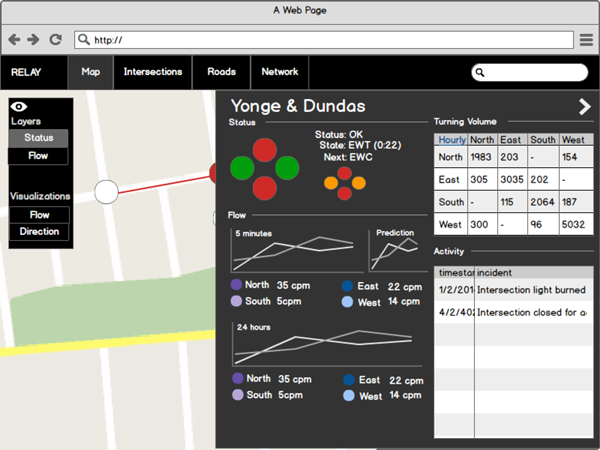
\includegraphics[scale=0.6]{figures/bals-3.png}
    \caption{Balsamiq mockup of the Relay dashboard.}
    \label{fig:bals-3}
  \end{centering}
\end{figure}

While the info box fulfills the need to browse intersections and provide quick snapshots of relevant intersection data, it was important for more advanced users to get an in depth look at this data, such that meaningful trends can be detected and acted upon.
It was necessary for these users - Traffic Engineers - to view metrics on intersection Location, Name, Type, State, In Flow, Out Flow, Predictions, and more.
To accommodate this large quantity of data, a dashboard was prototyped at this stage, setting a preliminary layout for each of the required metrics.
This dashboard slides across the screen from the right by pressing the arrow in the info box, and can then be toggled back and forth with the controls in the upper right corner of the screen.
A Balsamiq mockup of the dashboard can be found above in Figure \ref{fig:bals-3}.
As various intersections are selected on the map, the dashboard updates it's information to reflect that of the intended location.
Time-series graphs update in real-time as data feeds through the system, and an activity log hosts the history of noteworthy incidents at the selected intersection.

With these views on the Map screen prototyped in medium-fidelity, the design progressed into other areas of the application.
Moving through the global navigation buttons along the header, an Intersections page was mocked up.
The goal of this page is to give Traffic Engineers a holistic view on their network, as well as the ability to filter/search and target individual intersections.
This text-based search also allows for insight into any particular intersection by name, as well as the ability to find important groups of intersections or main arteries with many cross streets.
This is important because it allows users to locate intersections in two ways: spatially on the map, and now textually in the intersections table.
A mockup of the Intersections page is shown in Figure \ref{fig:bals-4}, with placeholder data in the intersections table. \\

\begin{figure}[htbp!]
  \begin{centering}
    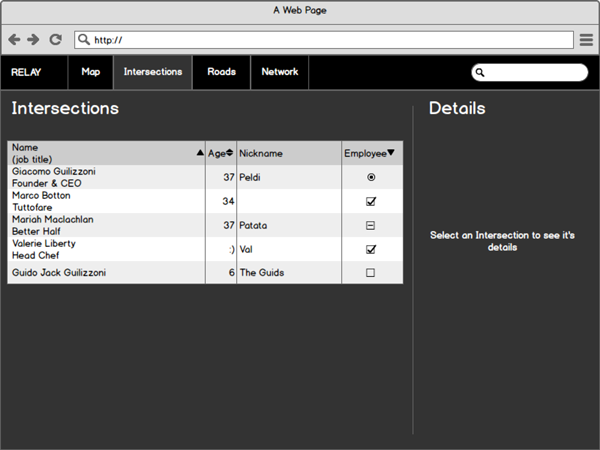
\includegraphics[scale=0.6]{figures/bals-4.png}
    \caption{Balsamiq mockup of the Intersections page.}
    \label{fig:bals-4}
  \end{centering}
\end{figure}

Finally, the medium-fidelity prototyping stage moved on to build out a layout and basic information for a Network page.
The intention of this page is to provide details similar to what would be shown in the info box or dashboard of an intersection, but for the entire network as a whole.
This allows Traffic Engineers to view, understand, diagnose, and make decisions for the network on a macro level, in addition to the finer look provided on a per intersection basis.
A mockup of the Network page is shown in Figure \ref{fig:bals-5}. \\

\begin{figure}[htbp!]
  \begin{centering}
    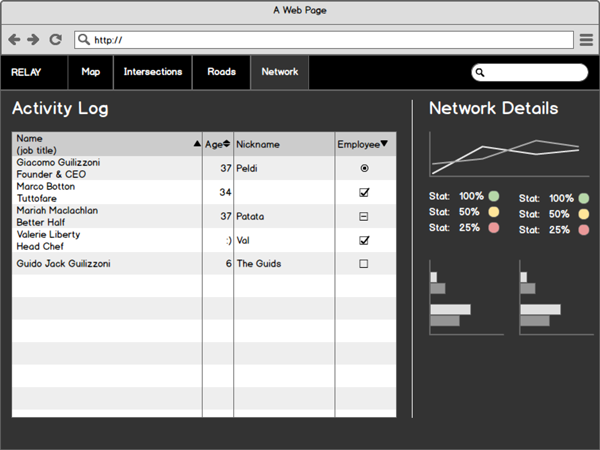
\includegraphics[scale=0.6]{figures/bals-5.png}
    \caption{Balsamiq mockup of the Network page.}
    \label{fig:bals-5}
  \end{centering}
\end{figure}

As can be seen in Figure \ref{fig:bals-5}, a large activity table is provided on the Network page, to highlight issues that occur at all intersections in the network.
These issues include accidents, power outages, abnormal volumes, and more.
Additional detail can be seen on the right hand side of the screen, with quantitative network data placed in charts and numerical tables, and colour-coding of network statuses explored at this stage.

Overall, the medium-fidelity prototyping stage was essential in moving the design of the Relay application forward towards its final state.
With functional requirements set in place, and now a strong roadmap of UI elements, navigation, page layout, and interactions to fulfill the requirements, the application was ready to be built in a high-fidelity form, as described in the following section.

\subsection{High-Fidelity Prototyping}
In preparation for the development of the Relay application, the design of the environment moved into a final high-fidelity prototyping phase.
This stage involved a major visual overhaul of the application, focusing on the definition of a unique design language to bring Relay together as a cohesive product.
Considerations at this stage include the creation of a custom grid structure, typography, colour, branding, the development of data visualization layers, and repurposing the search functionality in the app.
The high-fidelity design was done in Adobe Photoshop, Illustrator, and in the browser using HTML/CSS and JavaScript.
These tools allowed for highly accurate creation of assets, development of colour scheme, precise layout of visual elements, and more.

The branding for Relay was created in two main components: the logo, and the typesetting.
The logo is a custom glyph used in the application to denote the state of the signal at an intersection.
It contains four dots in a diamond pattern, with two fully-coloured dots positioned vertically, and two empty dots with a medium-weight stroke positioned horizontally.
In the application, this glyph would represent the flow of traffic in an East-West manner, while North-South traffic is halted at a red light.
This was selected to represent Relay as it both subtly represents what the application does, and provides important information to users in a modern and clean way.
The final Relay branding is shown in Figure \ref{fig:relay-logo}. \\ \\

\begin{figure}[htbp!]
  \begin{centering}
    
\includegraphics[scale=0.7]{figures/relay-logo.png}
    \caption{High-fidelity rendering of the Relay branding.}
    \label{fig:relay-logo}
  \end{centering}
\end{figure}

The typesetting was done to represent Relay in a way that would be clear, trustworthy, confident, readable, and modern.
The use of custom letter positioning through tracking and kerning methods aided this, while promoting clarity and confidence with the capitalization of each letter in the word.
Open Sans, a typeface that is freely available to the public, was utilized for the clean and readable aesthetic it provides.
As a sans-serif font set at a semi-bold weight, each letter is clear from any distance, at many sizes, on both screen and in print.
This also gives the branding a modern feel, as many serifed fonts are often associated with older, more classical and formal scenarios.

The high-fidelity design of the application itself began at a structural level, to set the basis for a consistent, coherent, and unique interface.
A grid structure was optimized for a 1440 x 900 pixel resolution screen - a common resolution on modern screens, and the dimensions of the screens used for the Symposium demo.
The grid was based upon units of 16 pixels, which was decided to be the lowest common denominator for icon and type sizing to ensure usability from many angles and distances.
With a grid structure in place, all following design decisions then had a reference point to follow from.
This aided in the purposeful use of negative spacing, symmetry, and balance of each screen composition.
The grid on a blank canvas is shown in Figure \ref{fig:dot-grid}. \\

\begin{figure}[htbp!]
  \begin{centering}
    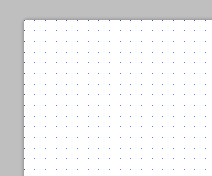
\includegraphics[scale=1]{figures/dot-grid.png}
    \caption{16 pixel grid foundation for the Relay user interface.}
    \label{fig:dot-grid}
  \end{centering}
\end{figure}

The first consideration in developing the design language for the application was the typography.
Just like the branding, the typography was intended to be clear and readable, but also neutral in tone.
Neutrality of the type allows for clear representation of the content itself, which is highly important in such a data-heavy application.
As a critical element of the user interface, particular attention was paid to hierarchy of type sizes and weights, all deriving from a smallest line-height of 16 pixels, used in small data labels and body.
The typeface Helvetica Neue was used, as it is well-known to provide very clear and readable text at many sizes, with a neutral tone.
Additionally, it is a common typeface used in the signage of many major cities around the world.
This gives the application a recognizable and associative feeling, which is especially important for an application that deals with traffic conditions in urban areas.
An example of an intersection name set in 24pt Helvetica Neue Bold is shown in Figure \ref{fig:name}. \\

\begin{figure}[htbp!]
  \begin{centering}
    
\includegraphics[scale=1]{figures/name.png}
    \caption{An intersection name set in 24pt Helvetica Neue Bold.}
    \label{fig:name}
  \end{centering}
\end{figure}

The high-fidelity prototyping process continued with the development of colour-scheme for the application.
Given the importance of visualizing data in the Relay app, it was decided that all non-data elements of the UI - the map, modular overlays, and header, for example - should be subdued and clearly grouped together as functionally similar elements.
To accomplish this, a black and white UI was established for all control elements, providing a clean environment for navigation, while vibrant, highly-saturated colours were used for charts and data layers.
This technique effectively created a high-contrast environment where areas that require visual focus, attention, and thought - i.e. the data - were the most salient elements on the screen, and any layout or navigational components were done in a clear black and white manner, similar to signage found on the streets of many major cities.
Therefore, all contextually similar elements were easily grouped and identifiable through their similarities or differences in colour.
An example of a chart showing the flow of traffic through an intersection over time is illustrated in Figure \ref{fig:chart}.
Notice the vibrancy of the coloured data, and its contrast with the structural page elements surrounding it. \\

\begin{figure}[htbp!]
  \begin{centering}
    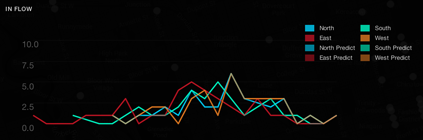
\includegraphics[scale=0.9]{figures/chart.png}
    \caption{A chart showing the flow of traffic through an intersection over time.}
    \label{fig:chart}
  \end{centering}
\end{figure}

The data visualization layers were next to be developed at the high-fidelity stage.
These visualizations took the form of heat maps, as well as quantitative, relative, and boolean glyphs, representing data on the Status, Flow, and Queue Length at a given intersection.
The first visualization layer, showing the Status of intersections, used small dot glyphs of different colour to display the boolean status of a light.
By overlaying a dot at each intersection, with a corresponding white or red colour to denote proper working condition vs. an error, such as a power outage, an easily digestible visualization was created.
This empowers Traffic Engineers to easily monitor their network, and to detect any anomalies that may have occurred.
A screenshot of the Status layer is shown in Figure \ref{fig:status}. \\

\begin{figure}[htbp!]
  \begin{centering}
    
\includegraphics[scale=0.9]{figures/status.png}
    \caption{A screenshot of the intersection Status data layer.}
    \label{fig:status}
  \end{centering}
\end{figure}

The second data layer to be designed was a heat map representing the flow of traffic through intersections.
This was accomplished on a per-intersection basis, and was intended to provide a macro view of the relative traffic density across areas of the city.
This view is most useful for those looking for an overview of general traffic conditions, such as a browsing Traffic Engineer, or a consumer looking to plan a route through the city.
A screenshot of the first Flow visualization layer is shown in Figure \ref{fig:flow-1}.

\begin{figure}[htbp!]
  \begin{centering}
    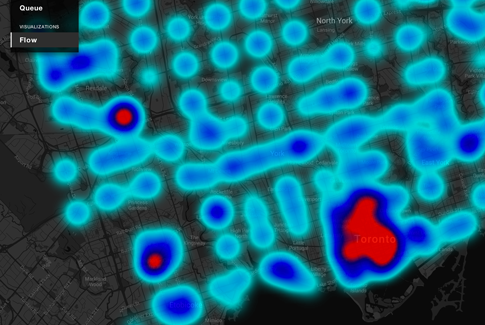
\includegraphics[scale=0.9]{figures/flow-1.png}
    \caption{A screenshot of the flow per-intersection heat map.}
    \label{fig:flow-1}
  \end{centering}
\end{figure}

Following this Flow visualization, a second implementation of traffic flow was developed, this time looking at flow between intersections, rather than at or through any particular intersection.
This was accomplished by taking predictive data from the controller, and approximating the position of cars along roadways given the knowledge of their entry and exit directions from each intersection.
Each car is plotted as a low-opacity glyph of concentric circles, with a bright green core, a lighter green exterior, and a soft blue outline, denoting the estimated nature of the position of any given car.
Given the large number of vehicles to be accounted for, a low opacity was selected for each individual glyph, so that as they overlap with one another, the intensity of the colour increases so as to illustrate the increasing density of traffic in an area.
A screenshot of the Flow between intersections data layer is shown in Figure \ref{fig:flow-2}.

\begin{figure}[htbp!]
  \begin{centering}
    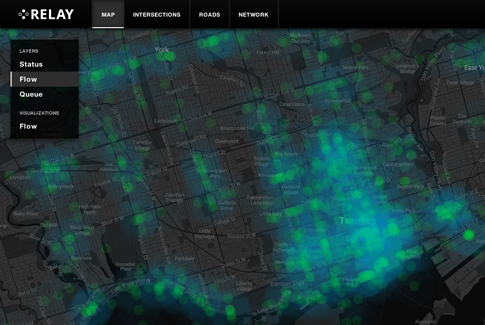
\includegraphics[scale=0.9]{figures/flow-2.png}
    \caption{A screenshot of the flow between intersections heat map.}
    \label{fig:flow-2}
  \end{centering}
\end{figure}

As can be seen in Figure \ref{fig:flow-2}, the natural visualization of major roadways and arteries through the cities is evident, which is an important result of this visualization.
A wide range of traffic patterns can be derived from this, thanks to the high-resolution of data points that give a continuous feel to the data, as opposed to the limited two-stage discrete options currently available through applications such as Google and Apple Maps.

Finally, the final visualization layer looked to showcase the data representing Queue Length or average wait time at an intersection.
The goal of this visualization was to produce glyphs that could show both quantitative measures, as well as give a sense of relative weighting between intersections.
A four-pronged glyph was developed, with three short prongs extending in the East, South, and West directions, while a variably sized prong extends to the North.
The length of the North prong corresponds to the average wait time at a given intersection, while the three shorter prongs are of equal length and serve as a stand for the quantitative North measure.
This creates a pseudo 3-dimensional effect, and gives the user a unique look at the changing landscape of queue lengths in the city - similar to how a city skyline may look with many tall buildings.
A screenshot of the Queue Length visualization layer is shown in Figure \ref{fig:queue}.

\begin{figure}[htbp!]
  \begin{centering}
    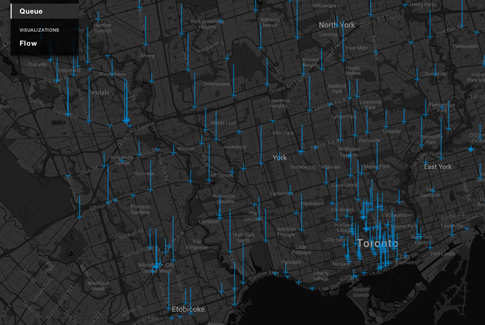
\includegraphics[scale=0.9]{figures/queue.png}
    \caption{A screenshot of the average queue length at each intersection.}
    \label{fig:queue}
  \end{centering}
\end{figure}

Following the design of the data visualization layers, the high-fidelity stage looked at the search functionality of the application, and focused attention on repurposing its form to better reflect its function.
Previous prototypes held the search bar in the header across all pages of the application.
This proved to be troublesome, as some pages did not require any search functionality, while the ones that did actually served as text-based filters within the context of the current page.
The high-fidelity design saw the removal of the search bar from the global navigation header, and into the upper section of the Intersections and Network pages.
This way, the text-based tables found on these pages could be easily searched/filtered, without the confusion of entering text into the global header, where a new page would be the expected result.

An additional feature that made its way through the high-fidelity phase is the Connection Status window.
This window is activated through the gear icon in the top right corner of the screen, and is useful for monitoring the status of the connection between the front-end and back-end of the application.
This window is positioned in the top-right of the screen so as to avoid covering any important visual elements, and is padded in from the top and right sides of the screen to maintain access to the dashboard toggle button.
The connection status window identifies where the data is coming from: either through a Web Socket or through the application's REST API.
It also identifies time since the last data update, both locally on a selected intersection, and globally over the entire network.
A screenshot of the Connection Status window is shown in Figure \ref{fig:connection}.

\begin{figure}[htbp!]
  \begin{centering}
    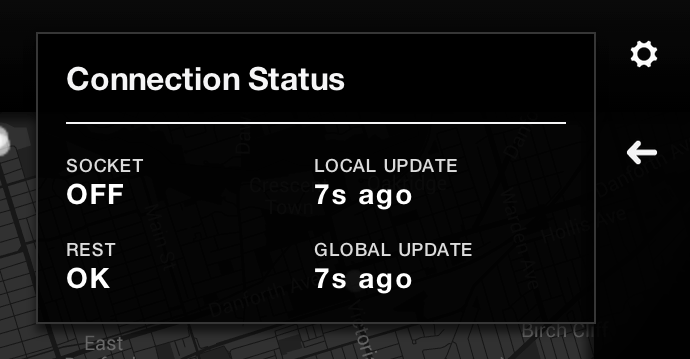
\includegraphics[scale=0.6]{figures/connection.png}
    \caption{A screenshot of the connection status window.}
    \label{fig:connection}
  \end{centering}
\end{figure}

Lastly, the intersection dashboard was refined at a high-fidelity stage.
The specific metrics contained in the dashboard were iterated on and refined from the medium-fidelity stage to accurately reflect the data coming from the back-end controller.
This involved splitting the Flow metric into In-Flow and Out-Flow at an intersection, showing the current and next intended State of the traffic lights, and providing a new Turn Predictions matrix, which gives the predicted quantity of cars moving through each permutation of turns based on stochastic data from the back-end.
In-line with the medium-fidelity prototype, the Activity Log is provided giving consideration to readability and interaction, with subtle hover states on individual table rows to improve salience of desired fields.
Additional information includes the Intersection ID and the Intersection Type, two identifiers that are often important to Traffic Engineers.
A screenshot of the high-fidelity dashboard is shown in Figure \ref{fig:dashboardt}. \\

\begin{figure}[htbp!]
  \begin{centering}
    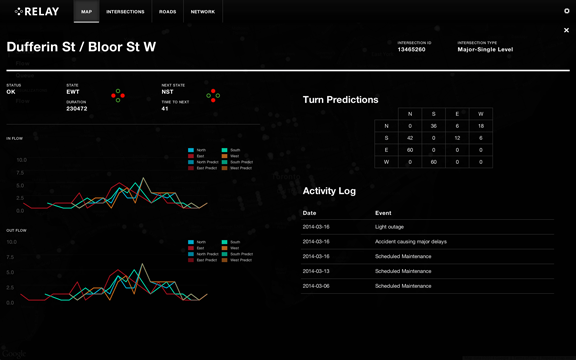
\includegraphics[scale=0.73]{figures/dashboard.png}
    \caption{A screenshot of the Relay intersection dashboard.}
    \label{fig:dashboardt}
  \end{centering}
\end{figure}

With these elements in place, the final developmental/functional touches to the Relay application were ready to be built for the demo, as showcased on Symposium day.
As a unit, the application is held together using the modular design elements described above, which makes the application easily scalable and modifiable for individual implementations or changing metrics and requirements.
With a unique and well-defined design language established, further extrapolations of this implementation have a library of best practices and UI elements that can be carried forward into new scenarios.

\section{Front End}

\subsection{Deep End}
\subsection{Design Research}

\subsection{Design Process}

\subsection{Application Architecture}

\subsubsection{Framework Selection}

\subsubsection{Mapping Library Selection}

\subsubsection{Visualization Library Selection}

\section{Back End}

\section{Deep End}

\subsection{Learning in Relay}
\subsubsection{Design Parameter Updates}

Each agent within the system has multiple design parameters that will constantly update. With each cycle -- behaviour change -- predictions and estimations are made to recalculate these parameters. 
The following sections explain how these variables are learned and updated.

\subsubsection{Time Delay Estimation}
The first important parameter needed to calculate predictions is the time delay estimate between two agents. 
This can be thought of as the estimated time to travel from one intersection to a neighbouring one. 
However, this is not a fixed time, so the delay is modelled using a gamma distribution, as discussed previously. 

The first step in performing this estimation, is determining which portion of the downstream signal is relevant – meaning what part of the signal should be considered for the estimation. 
This is required because it must match the departing signal from the upstream intersection. 
To extract the downstream signal, an upstream sub-signal is first selected. It was determined that the most efficient way to do this is to this is to select the upstream departure signal created by the previous behaviour cycle. 
To ensure that events are not missed, the downstream signal is determined by time-shifting the upstream signal by the expected value of the previous time delay distribution, and a small buffer is added to each end.

After the two signals are extracted, the estimation process can be performed. 
Equation [time-delay-opt] outlines the optimization problem, using least squares. 
The goal of this optimization is to convolve the departure signal with a gamma distribution to best estimate the downstream arrival signal -- to minimize the difference between the real signal and estimated. 
The design parameters are: shape, location, scale, and gain. 
The first three are what control the parameters of the distribution and the last is a measure of the change in cars while traversing the road -- to capture the effect of cars turning onto or off of the road on side streets.

Below, in Figure \ref{fig:time-delay-est}, an example estimate is performed. 
Two signals are provided (departure is pre-calculated within the agent and not shown here), trimmed, and then the optimization procedure is executed. 
The resulting distribution is overlaid on the downstream signal and estimated time delay gamma plotted above.

\begin{figure}[htbp!]
  \begin{centering}
    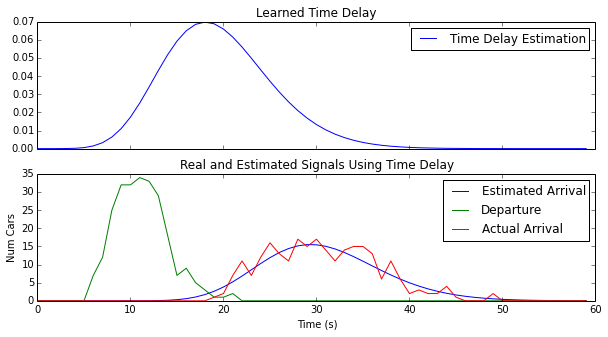
\includegraphics[scale=0.75]{figures/time-delay-est.png}
    \caption{Example time delay estimation.}
    \label{fig:time-delay-est}
  \end{centering}
\end{figure}


\subsubsection{Updating Intra-Agent Behaviour Graphs}
The second important piece in generating signal predictions is learning the intra-agent graph probabilities. 
These represent the likelihood of a signal to travel along this edge during the executed behaviours cycle.

\paragraph{Behaviour Probability Matrix (BPM)}
Figure \ref{fig:BPM-example} provides a visualization of this to help parse this idea. 
The matrix represents how these edge probabilities are used within the system; in the matrix, departing nodes are along the columns and entering along the rows -- $p_{02}$ would represent entering node 0 and exiting node 2. 
It is seen in the diagram that an event occurring at node 0 has a 60\% likelihood of exiting node 2, for this behaviour.
It is important to not that edges that are not traversable will always have a probability of 0. 
Essentially, this probability matrix is used to split an entering signal into components, to then be combined with other estimates in a departing signal. 
This estimated signal is then used in combination with the time delay estimation to predict expected traffic, which will be discussed further in the following section.

\begin{figure}[htbp!]
  \begin{centering}
    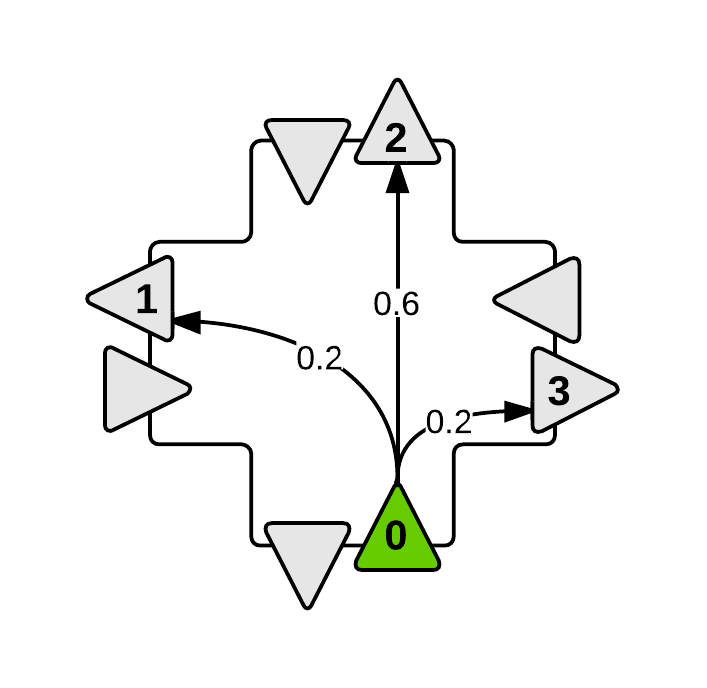
\includegraphics[scale=0.3]{figures/BPM-example.png}
    \caption{Example intra-agent edge probabilities for node 0.}
    \label{fig:BPM-example}
  \end{centering}
\end{figure}


\[
{BPM} =
    \begin{bmatrix}
    p_{00} & p_{01} & p_{02} & p_{03} \\
    p_{10} & p_{11} & p_{12} & p_{13} \\
p_{20} & p_{21} & p_{22} & p_{23} \\
p_{30} & p_{31} & p_{32} & p_{33} \\
    \end{bmatrix}
\]

\paragraph{Learning Probabilities}

\paragraph{Updating BPMs}
After the optimization procedure has arrived at a solution, the existing BPM must be updated. 
It would be unwise to directly use the newly calculated BPM as temporary inhibitors to traffic flow, such as accidents, can greatly skew results. 
Therefore, a learning parameter is used to update existing probabilities, seen in Equation \ref{eqn:BPM-update}. 
This can be tuned, on an agent-by-agent basis, to alter how quickly these values are modified and adapt – an average of the two values is a good starting point, to enable quick transitions, while remaining relatively stable. 
In \ref{eqn:BPM-update}, $i$ represents the agents ID and $BPM_{est}^{i}$ is the newly estimated behaviour probability matrix for that agent.

\begin{equation}
    BPM_{new}^{i} = \alpha^{i} \times BPM_{old}^{i} + (1 - \alpha^{i}) \times BPM_{est}^{i}
    \label{eqn:BPM-update}
\end{equation}t

\newpage
\chapter{Design Testing and Validation}

\section{Front End}

\section{Back End}

\section{Deep End}

\newpage
\chapter{Recommended Design Modifications}

\newpage
\chapter{Timeline and Project Management}

\newpage
\section{Conclusion}

\newpage
\addcontentsline{toc}{section}{References}

\bibliographystyle{IEEEtran}

\bibliography{bib}

\end{document}
